\section{The WKB Approximation}
\subsection*{Sol. 1}
\begin{align*}
    \int_0^{a/2}\sqrt{2m(E_n-V_0)}dx + 
    \int_{a/2}^a\sqrt{2mE_n}dx = n\pi \hbar
\end{align*}
\begin{align*}
    \sqrt{2m(E_n-V_0)}\frac{a}{2}
    +
    \sqrt{2mE_n}\frac{a}{2}=n\pi \hbar
\end{align*}
\begin{align*}
    2m(E_n-V_0)+2mE_n
    +2\sqrt{4m^2(E_n-V_0)E_n}
    =\frac{4n^2\pi^2\hbar^2}{a^2}
\end{align*}
\begin{align*}
    2E_n-V_0
    +
    2\sqrt{(E_n-V_0)E_n}
    =4E^0_n
\end{align*}
\begin{align*}
    4(E_n-V_0)E_n = 
    4E_n^2-4E_n(4E_n^0+V_0)+(4E_n^0+V_0)^2
\end{align*}
\begin{align*}
    E_n = \frac{(4E^0_n+V_0)^2}{16 E_n^0}
\end{align*}
If $V_0$ is very small or $n$ is very large,
\begin{align*}
    \frac{(4E^0_n+V_0)^2}{16 E_n^0}\approx
    \frac{1}{16E_n^0}
    (16(E_n^0)^2+8E_n^0V_0)
    =E_n^0+\frac{V_0}{2}.
\end{align*}

\subsection*{Sol. 2}
\begin{enumerate}
    \item 
    \begin{align*}
    \frac{d^2}{dx^2}e^{if(x)/\hbar} 
    = \frac{i}{\hbar}
    f''(x)e^{if(x)/\hbar} 
    -
    \frac{1}{\hbar^2}
    (f'(x))^2e^{if(x)/\hbar} 
    = -\frac{p^2}{\hbar^2}
    e^{if(x)/\hbar} 
\end{align*}
\begin{align*}
    i\hbar f'' - (f')^2 + p^2 = 0
\end{align*}
\item 
\begin{align*}
    i\hbar(f_0''+\hbar f_1'' + \hbar^2f_2'')
    -(f_0'+\hbar f_1'+\hbar^2 f_2')^2
    +p^2 = 0
\end{align*}
\begin{align*}
    p^2 = (f_0')^2
\end{align*}
\begin{align*}
    if_0''-2f_0'f_1' = 0
\end{align*}
\begin{align*}
    if_1''-2f_0'f_2'-(f_1')^2=0
\end{align*}
\item 
\begin{align*}
    f_0 = \pm \int p
\end{align*}
\begin{align*}
    f_1' = \frac{if_0''}{2f_0'}
    \Rightarrow 
    f_1 = 
    \frac{i}{2}\log f_0'
    =\frac{i}{2}\log (\pm p)
\end{align*}
$$
f_1^+ = \frac{i}{2}\log (p)
$$
$$
f_1^- = \frac{i}{2}\log (p) - \frac{1}{2}n\pi,
$$
where $n$ is an odd number.
Thus,
\begin{align*}
    \psi(x)\approx &
    \exp\left[
    i(\pm \int p + \hbar \frac{i}{2}\log p)/\hbar
    \right]\\
    =&
    \exp\left[
    \pm \frac{i}{\hbar}\int p 
    \right]
    \exp[\frac{-1}{2}\log p]\\
    \propto&
    \frac{C}{\sqrt{|p|}}
    \exp\left[
    \pm \frac{i}{\hbar}\int p 
    \right]
\end{align*}


\end{enumerate}


\subsection*{Sol. 3} 
\begin{align*}
    \gamma =& \frac{1}{\hbar}
    \int_0^{2a}|\sqrt{2m(E-V_0)}|dx\\
    =&
    \frac{1}{\hbar}
    \sqrt{2m(V_0-E)}2a
\end{align*}
\begin{align*}
    T \sim
    \exp\left[-\frac{4a}{\hbar}
    \sqrt{2m(V_0-E)}\right]
\end{align*}
Compare with prob2.33, if $a$ and $V_0$ are large, then

\begin{align*}
    T^{-1}=&
    1+\frac{V_0^2}{4E(V_0-E)}
    \sinh^2\left(\frac{2a}{\hbar}\sqrt{2m(V_0-E)}\right)\\
    \approx&
    1+\frac{V_0^2}{4E(V_0-E)}
    \frac{1}{4}\exp
    \left(\frac{4a}{\hbar}\sqrt{2m(V_0-E)}\right)\\
    \sim &
    \exp
    \left(\frac{4a}{\hbar}\sqrt{2m(V_0-E)}\right)
\end{align*}

\subsection*{Sol. 4}
For \ce{U^{238}},
$$
r_1=(1.25)\times 238^{1/3} \approx 7.746fm
$$
$m_p = 
238050786.9 \mu u,$ 
$m_d=
234043599.8\mu u,$ 
$m_\alpha=4002603.25413\mu u.$
$$
E\approx 6.841\times 10^{-13}J = 4.27MeV.
$$
$$
v\approx 1.43476\times 10^7m/s
$$
$$
\gamma \approx 1.980\times \frac{90}{\sqrt{4.27}} - 1.485\times \sqrt{90\times 7.746}\approx 47.029
$$
$$
\tau = \frac{2\times 7.746\times 10^{-15}}
{1.43476\times 10^7}
e^{2\times 47.029} 
\approx 2.414\times 10^{12} yrs.
$$


For \ce{Po^{212}},
$$
r_1=(1.25)\times 212^{1/3} \approx 7.453fm
$$
$m_p = 
211988868.0 \mu u,$ 
$m_d=
207976652.0\mu u,$ 
$m_\alpha=4002603.25413\mu u.$
$$
E\approx 1.435\times 10^{-12}J = 8.954MeV.
$$
$$
v\approx 2.0777254\times 10^7m/s
$$
$$
\gamma \approx 1.980\times \frac{82}{\sqrt{8.954}} - 1.485\times \sqrt{82\times 7.453}\approx 17.546
$$
$$
\tau = \frac{2\times 7.453\times 10^{-15}}
{2.0777254\times 10^7}
e^{2\times 17.546} 
\approx 1.25\mu s.
$$

\subsection*{Sol. 5}
$$
a = \frac{E_g}{eE_0}
$$
\begin{align*}
    \gamma =&
    \frac{1}{\hbar}
    \int_0^{\frac{E_g}{eE_0}}
    \sqrt{2m(E_g - eE_0x)}dx\\
    =&
    \frac{1}{\hbar}
    \frac{2}{3(-2meE_0)}
    (2mE_g - 2meE_0x)^{3/2}
    \bigg|^{\frac{E_g}{eE_0}}_0\\
    =&
    \frac{1}{\hbar}
    \frac{1}{3meE_0}
    (2mE_g)^{3/2}
\end{align*}
$$
T\sim \exp\left(
\frac{-2}{\hbar}
    \frac{1}{3meE_0}
    (2mE_g)^{3/2}
\right)
$$

\subsection*{Sol. 6}
\begin{enumerate}
    \item 
    \begin{align*}
        V(x) = \begin{cases}
        mgx, \; x>0\\
        \infty,\; x<0
        \end{cases}
    \end{align*}
    \item 
    For $x>0,$
    \begin{align*}
        -\frac{\hbar^2}{2m}
        \frac{d^2}{dx^2}
        \psi + mgx\psi = E\psi
    \end{align*}
    Let $z = ax+b,$ then 
    \begin{align*}
        -\frac{\hbar^2}{2m}
        a^2\frac{d^2}{dz^2}
        \psi + mg\frac{z-b}{a}\psi = E\psi
    \end{align*}
    \begin{align*}
        \frac{d^2}{dz^2}\psi
        =\frac{-2m}{\hbar^2a^2}
        \left(
        -\frac{mg}{a}z + E+\frac{mgb}{a}
        \right)\psi
    \end{align*}
    Let $
    a=\left(\frac{2m^2g}{\hbar^2}\right)^{1/3},
    $
    $b=-\frac{Ea}{mg},$ then
    $$
    \psi(x) = A\operatorname{Ai}(ax+b).
    $$
    \item 
    $\psi(0)=0=\operatorname{Ai}(b)$
    $$
    E=\frac{-mgz_0}{a}
    =8.81\times 10^{-23}J, \; 1.54\times 10^{-22}J, \;
    2.08\times 10^{-22}J, \; 2.56\times 10^{-22}J.
    $$
    \item 
    $$
    1.148\times 10^{-13}eV.
    $$
    $$
    2\langle T\rangle
    =mg\langle x\rangle
    $$
    $$
    \langle x \rangle
    =\frac{2E}{3mg}
    \approx 1.37mm
    $$
\end{enumerate}

\subsection*{Sol. 7}
\begin{enumerate}
    \item 
    $$
    mgx_2 = E 
    $$
    \begin{align*}
        \int_0^{\frac{E}{mg}}
        \sqrt{2m(E - mgx)}dx = \left( n -\frac{1}{4}\right)\pi\hbar
    \end{align*}
    \begin{align*}
        \frac{2}{3(-2m^2 g)}
        (2mE - 2m^2 gx)^{3/2}\bigg|^{\frac{E}{mg}}_0=
        \frac{1}{3m^2 g}(2mE)^{3/2}
    \end{align*}
    \begin{align*}
        E_n = \frac{1}{2m}
        \left[
        3m^2 g(n-1/4)\pi\hbar
        \right]^{2/3}
    \end{align*}
    \item 
    $$
    E_1=8.74\times 10^{-23}J,\;
    E_2=1.54\times 10^{-22}J,\;
    E_3=2.08\times 10^{-22}J,\;
    E_4 = 2.55\times 10^{-22}J.
    $$
    \item 
    \begin{align*}
        \frac{2}{3mg}\frac{1}{2m}
        \left[
        3m^2 g(n-1/4)\pi\hbar
        \right]^{2/3}\geq 1
        \Rightarrow
        (3m^2g)^{3/2}
        \frac{1}{3m^2 g\pi\hbar}+\frac{1}{4}
        \approx 1.64\times 10^{33}.
    \end{align*}
    
\end{enumerate}

\subsection*{Sol. 8}
\begin{align*}
    \frac{1}{2}m\omega^2x^2 = E
    \Rightarrow
    x_1=-\sqrt{\frac{2E}{m\omega^2}},\;
    x_2=\sqrt{\frac{2E}{m\omega^2}}
\end{align*}
\begin{align*}
    \int_{x_1}^{x_2}
    \sqrt{2m(E-\frac{1}{2}m\omega^2x^2)}
    dx
    =&
    x\sqrt{2mE-m^2\omega^2x^2}
    -2mE
    \frac{1}{m\omega}
    \arcsin\frac{-2m^2\omega^2 x}{\sqrt{4m^2\omega^2 2mE}}
    \bigg|^{\sqrt{\frac{2E}{m\omega^2}}}_0\\
    =&
    \frac{\pi E_n}{\omega}
    =\left(n-\frac{1}{2}\right)\pi\hbar 
\end{align*}
\begin{align*}
    E_n = 
    \left(n-\frac{1}{2}\right)\omega\hbar,\;
    n=1,2,3,\dots
\end{align*}

\subsection*{Sol. 9}
\begin{enumerate}
    \item 
    \begin{align*}
        x_2 = &
        \sqrt{\frac{2}{m\omega^2}
        \left(n+\frac{1}{2}\right)\omega\hbar }\\
        = & 
        \sqrt{\frac{2\hbar}{m\omega}
        \left(n+\frac{1}{2}\right) }
    \end{align*}
    \item 
    \begin{align*}
        V_{lin}(x)
        =\frac{1}{2}m\omega^2x_2^2 + 
        m\omega^2 x_2(x-x_2)
        =m\omega^2 x_2x
        -\frac{1}{2}m\omega^2x_2^2
    \end{align*}

    
    \begin{align*}
        \frac{\frac{1}{2}m\omega^2 (x_2+d)^2
        -\left(
        m\omega^2 x_2(x_2+d)
        -\frac{1}{2}m\omega^2x_2^2
        \right)}
        {\frac{1}{2}m\omega^2 x_2^2}
        =0.01
    \end{align*}
    \begin{align*}
        \frac{1}{2}m\omega^2x^2_2+
        m\omega^2 x_2d
        +\frac{1}{2}m\omega^2 d^2
        -m\omega^2 x_2^2
        -m\omega^2 x_2d
        +\frac{1}{2}m\omega^2 x_2^2
        =0.01 
        \frac{1}{2}m\omega^2 x_2^2
    \end{align*}
    \begin{align*}
         d
        =0.1 
         x_2
    \end{align*}
    \item 
    \begin{align*}
        \alpha d
        =&\left(
        \frac{2m}{\hbar^2}
        m\omega^2
        x_2
        \right)^{1/3}
        0.1 
        x_2\\
        =&
        \left(
        2\frac{4(n+1/2)^2}{x_2^4}
        x_2
        \right)^{1/3}
        0.1 
        x_2
    \end{align*}
    \begin{align*}
        (n+\frac{1}{2})^{2}
        \geq
        (5/0.1)^3/8
        \Rightarrow n\geq 124.5
    \end{align*}
    
\end{enumerate}
\subsection*{Sol. 10}
For the downward sloping,
\begin{align*}
    \psi(x)=
    \begin{cases}
    \frac{1}{\sqrt{|p(x)|}}D\exp\left[
    -\frac{1}{\hbar}\int_x^0|p(x')|dx'
    \right],\; x<0\\
    \frac{1}{\sqrt{p(x)}}
    \left(B\exp\left[
    \frac{i}{\hbar}\int_0^x|p(x')|dx'
    \right]
    +
    C\exp\left[
    -\frac{i}{\hbar}\int_0^x|p(x')|dx'
    \right]
    \right),\; x>0.
    \end{cases}
\end{align*}
\begin{align*}
    p(x)=\hbar(-\alpha)^{3/2}\sqrt{x}
\end{align*}
In overlap region 1,
\begin{align*}
    \int_x^0|p(x')|dx'\approx 
    \hbar(-\alpha)^{3/2}\frac{2}{3}(-x)^{3/2}
    =\frac{2}{3}\hbar(\alpha x)^{2/3}
\end{align*}
\begin{align*}
    \psi(x)=\frac{D}{\sqrt{\hbar}(-\alpha)^{3/4}x^{1/4}}
    \exp\left[-
    \frac{2}{3}(\alpha x)^{2/3}
    \right]
\end{align*}
Using the asymptotic form of the Airy function
\begin{align*}
    \psi_p(x)=\frac{a}{2\sqrt{\pi}(\alpha x)^{1/4}}
    \exp\left[-\frac{2}{3}(\alpha x)^{3/2}\right]
    +
    \frac{b}{\sqrt{\pi}(\alpha x)^{1/4}}
    \exp\left[\frac{2}{3}(\alpha x)^{3/2}\right]
\end{align*}
$b=0,$
$a=\sqrt{\frac{-4\pi}{\alpha \hbar}}D.$

In overlap region 2,
\begin{align*}
    \int_0^x|p(x')|dx'\approx 
    \hbar(-\alpha)^{3/2}\frac{2}{3}x^{3/2}
    =\frac{2}{3}\hbar(-\alpha x)^{2/3}
\end{align*}

\begin{align*}
    \psi(x)=\frac{1}{\sqrt{\hbar}(-\alpha)^{3/4}x^{1/4}}
    \left(B\exp\left[
    i\frac{2}{3}(-\alpha x)^{2/3}
    \right]
    +
    C\exp\left[
    -i\frac{2}{3}(-\alpha x)^{2/3}
    \right]
    \right)
\end{align*}

\begin{align*}
    \psi_p(x)=&\frac{a}{\sqrt{\pi}(-\alpha x)^{1/4}}
    \sin\left[
    \frac{2}{3}
    (-\alpha x)^{3/2}+\frac{\pi}{4}
    \right]\\
    =&
    \frac{a}{\sqrt{\pi}(-\alpha x)^{1/4}}
    \frac{1}{2i}
    \left[
    \exp\frac{i\pi}{4}
    \exp\left[
    i\frac{2}{3}
    (-\alpha x)^{3/2}
    \right]
    -
    \exp\frac{-i\pi}{4}
    \exp\left[
    -i\frac{2}{3}
    (-\alpha x)^{3/2}
    \right]
    \right]
\end{align*}
\begin{align*}
    \frac{B}{\sqrt{\hbar}(-\alpha)^{3/4}x^{1/4}}
    =\frac{a}{\sqrt{\pi}(-\alpha x)^{1/4}2i}e^{i\pi /4},\;
    \frac{C}{\sqrt{\hbar}(-\alpha)^{3/4}x^{1/4}}
    =\frac{-a}{\sqrt{\pi}(-\alpha x)^{1/4}2i}e^{-i\pi /4}
\end{align*}
\begin{align*}
    B = -ie^{i\pi /4}D,\;
    C =ie^{-i\pi /4}D.
\end{align*}
The WKB wavefunction for the downward sloping is
\begin{align*}
    \psi(x)=
    \begin{cases}
    \frac{D}{\sqrt{|p(x)|}}\exp\left[
    -\frac{1}{\hbar}\int_x^{x_1}|p(x')|dx'
    \right],\; x<x_1\\
    \frac{2D}{\sqrt{p(x)}}
    \sin\left[
    \frac{1}{\hbar}\int_{x_1}^x|p(x')|dx'
    +\frac{\pi}{4}
    \right],\; x>x_1.
    \end{cases}
\end{align*}

\subsection*{Sol. 11}
Move $x_1$ to the origin, then
\begin{align*}
    \psi(x)\approx 
    \frac{C}{\sqrt{\hbar}\alpha^{3/4}x^{1/4}}
    e^{\frac{2}{3}(\alpha x)^{3/2}} + \frac{D}{\sqrt{\hbar}\alpha^{3/4}x^{1/4}}
    e^{-\frac{2}{3}(\alpha x)^{3/2}}
\end{align*}
Compare with the large-z asymptotic forms,
\begin{align*}
    \frac{D}{\sqrt{\hbar}\alpha^{3/4}x^{1/4}}=\frac{a}{2\sqrt{\pi}(\alpha x)^{1/4}},\;
    \frac{C}{\sqrt{\hbar}\alpha^{3/4}x^{1/4}}=\frac{b}{\sqrt{\pi}(\alpha x)^{1/4}}
\end{align*}
\begin{align*}
    a =
    \sqrt{\frac{4\pi}{\alpha\hbar}}D
    , \;
    b =
    \sqrt{\frac{\pi}{\alpha\hbar}}C
\end{align*}
For the overlap region 1
\begin{align*}
    \psi(x) = 
    \frac{1}{\sqrt{\hbar}\alpha^{3/4}(-x)^{1/4}}
    [Ae^{i\frac{2}{3}(-\alpha x)^{3/2}}+
    Be^{-i\frac{2}{3}(-\alpha x)^{3/2}}]
\end{align*}
The asymptotic form for large negative z is then 
\begin{align*}
    \psi_p(x)=&
    \frac{a}{\sqrt{\pi}(-\alpha x)^{1/4}}\sin\left[
    \frac{2}{3}(-\alpha x)^{3/2}+\frac{\pi}{4}
    \right]
    +
    \frac{b}{\sqrt{\pi}(-\alpha x)^{1/4}}\cos\left[
    \frac{2}{3}(-\alpha x)^{3/2}+\frac{\pi}{4}
    \right]\\
    =&
    \frac{a}{\sqrt{\pi}(-\alpha x)^{1/4}}
    \frac{1}{2i}[
    e^{i\pi/4}e^{i\frac{2}{3}(-\alpha x)^{3/2}}
    -
    e^{-i\pi/4}e^{-i\frac{2}{3}(-\alpha x)^{3/2}}
    ]\\
    &+
    \frac{b}{\sqrt{\pi}(-\alpha x)^{1/4}}
    \frac{1}{2}[
    e^{i\pi/4}e^{i\frac{2}{3}(-\alpha x)^{3/2}}
    +
    e^{-i\pi/4}e^{-i\frac{2}{3}(-\alpha x)^{3/2}}
    ]
\end{align*}

\begin{align*}
    \frac{a}{\sqrt{\pi}(-\alpha x)^{1/4}}
    \frac{1}{2i}e^{i\pi /4}
    +
    \frac{b}{\sqrt{\pi}(-\alpha x)^{1/4}}
    \frac{1}{2}e^{i\pi /4}
    =\frac{A}{\sqrt{\hbar}\alpha^{3/4}(-x)^{1/4}}
\end{align*}
\begin{align*}
    \frac{a}{\sqrt{\pi}(-\alpha x)^{1/4}}
    \frac{-1}{2i}e^{-i\pi /4}
    +
    \frac{b}{\sqrt{\pi}(-\alpha x)^{1/4}}
    \frac{1}{2}e^{-i\pi /4}
    =\frac{B}{\sqrt{\hbar}\alpha^{3/4}(-x)^{1/4}}.
\end{align*}

\begin{align*}
    -iD
    e^{i\pi /4}
    +
    C
    \frac{1}{2}e^{i\pi /4}
    =A
\end{align*}
\begin{align*}
    iD
    e^{-i\pi /4}
    +
    C
    \frac{1}{2}e^{-i\pi /4}
    =B
\end{align*}
Write the middle part 
\begin{align*}
    \psi(x)
    =&\frac{1}{\sqrt{|p(x)|}}
    \left[
    Ce^{\frac{1}{\hbar}\int_{x_1}^{x_2}|p(x')|dx'}
    e^{\frac{-1}{\hbar}\int_{x}^{x_2}|p(x')|dx'}
    +
    De^{-\frac{1}{\hbar}\int_{x_1}^{x_2}|p(x')|dx'}
    e^{\frac{1}{\hbar}\int_{x}^{x_2}|p(x')|dx'}
    \right]\\
    =&
    \frac{1}{\sqrt{|p(x)|}}
    \left[
    Ce^\gamma
    e^{\frac{-1}{\hbar}\int_{x}^{x_2}|p(x')|dx'}
    +
    De^{-\gamma}
    e^{\frac{1}{\hbar}\int_{x}^{x_2}|p(x')|dx'}
    \right]
\end{align*}


Now move $x_2$ to the origin, then in the overlap region 1

\begin{align*}
    \psi(x)=\frac{1}{\sqrt{\hbar}(-\alpha)^{3/4}(-x)^{1/4}}
    \left[
    Ce^\gamma
    e^{-\frac{2}{3}(\alpha x)^{3/2}}
    +
    De^{-\gamma}
    e^{\frac{2}{3}(\alpha x)^{3/2}}
    \right]
\end{align*}
The large asymptotic form
\begin{align*}
    \psi_p(x)
    =\frac{a'}{2\sqrt{\pi}(\alpha x)^{1/4}}
    e^{-\frac{2}{3}(\alpha x)^{3/2}}
    +
    \frac{b'}{\sqrt{\pi}(\alpha x)^{1/4}}
    e^{\frac{2}{3}(\alpha x)^{3/2}}
\end{align*}
\begin{align*}
    \frac{Ce^\gamma}{\sqrt{\hbar}(-\alpha)^{3/4}(-x)^{1/4}}    
    =\frac{a'}{2\sqrt{\pi}(\alpha x)^{1/4}}
\end{align*}
\begin{align*}
    \frac{De^{-\gamma}}{\sqrt{\hbar}(-\alpha)^{3/4}(-x)^{1/4}}
    =\frac{b'}{\sqrt{\pi}(\alpha x)^{1/4}}
\end{align*}
\begin{align*}
    a'=
    \sqrt{\frac{4 \pi}{-\alpha\hbar}}
    Ce^\gamma
\end{align*}
\begin{align*}
    b'=
    \sqrt{\frac{\pi}{-\alpha \hbar}}
    De^{-\gamma}
\end{align*}
For the overlap region 2
\begin{align*}
    \psi(x)=
    \frac{1}{\sqrt{\hbar}(-\alpha)^{3/4}(x)^{1/4}}
    Fe^{i\frac{2}{3}\hbar(-\alpha x)^{3/2}}
\end{align*}
\begin{align*}
    \psi_p(x)=&
    \frac{a'}{\sqrt{\pi}(-\alpha x)^{1/4}}\sin\left[
    \frac{2}{3}(-\alpha x)^{3/2}+\frac{\pi}{4}
    \right]
    +
    \frac{b'}{\sqrt{\pi}(-\alpha x)^{1/4}}\cos\left[
    \frac{2}{3}(-\alpha x)^{3/2}+\frac{\pi}{4}
    \right]\\
    =&
    \frac{a'}{\sqrt{\pi}(-\alpha x)^{1/4}}
    \frac{1}{2i}[
    e^{i\pi/4}e^{i\frac{2}{3}(-\alpha x)^{3/2}}
    -
    e^{-i\pi/4}e^{-i\frac{2}{3}(-\alpha x)^{3/2}}
    ]\\
    &+
    \frac{b'}{\sqrt{\pi}(-\alpha x)^{1/4}}
    \frac{1}{2}[
    e^{i\pi/4}e^{i\frac{2}{3}(-\alpha x)^{3/2}}
    +
    e^{-i\pi/4}e^{-i\frac{2}{3}(-\alpha x)^{3/2}}
    ]
\end{align*}
\begin{align*}
    \frac{a'}{\sqrt{\pi}(-\alpha x)^{1/4}}
    \frac{1}{2i}e^{i\pi /4}
    +
    \frac{b'}{\sqrt{\pi}(-\alpha x)^{1/4}}
    \frac{1}{2}e^{i\pi /4}=
    \frac{F}{\sqrt{\hbar}(-\alpha)^{3/4}(x)^{1/4}}
\end{align*}
\begin{align*}
    \frac{-a'}{\sqrt{\pi}(-\alpha x)^{1/4}}
    \frac{1}{2i}e^{-i\pi /4}
    +
    \frac{b'}{\sqrt{\pi}(-\alpha x)^{1/4}}
    \frac{1}{2}e^{-i\pi /4}=0
\end{align*}
\begin{align*}
    -iCe^\gamma
    e^{i\pi /4}
    +
    De^{-\gamma}
    \frac{1}{2}e^{i\pi /4}=
    F
\end{align*}
\begin{align*}
    i
    Ce^{\gamma}
    +
    De^{-\gamma}
    \frac{1}{2}=0
\end{align*}
Therefore,
\begin{align*}
    C = \frac{F}{2}e^{-\gamma}e^{-i\pi/4}i,\;
    D = e^\gamma e^{-i\pi/4}F
\end{align*}
\begin{align*}
    A = &-ie^\gamma F + \frac{1}{2}\frac{F}{2}e^{-\gamma}i\\
    =&i\left(-e^\gamma + \frac{e^{-\gamma}}{4}\right)F
\end{align*}
\begin{align*}
    \frac{|F|^2}{|A|^2}
    =&\frac{1}{\left(-e^\gamma + \frac{e^{-\gamma}}{4}\right)^2}.
\end{align*}
When $\gamma$ is large,
\begin{align*}
    \frac{|F|^2}{|A|^2}\sim e^{-2\gamma}.
\end{align*}
\subsection*{Sol. 12}
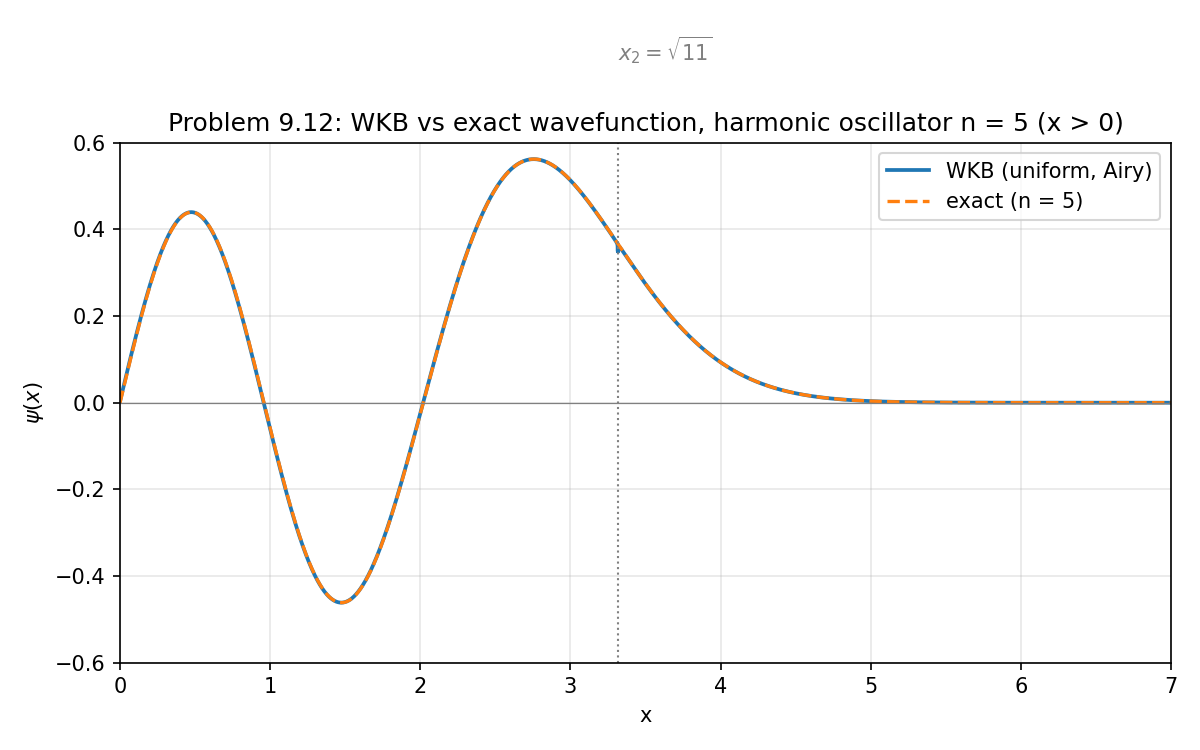
\includegraphics[width=0.8\textwidth,valign=t]{fig/prob9.12.png}

\subsection*{Sol. 13}
\begin{align*}
    2\int_0^{x_2}
    \sqrt{2m(E-\alpha x^\nu)}dx
    =(n-\frac{1}{2})\pi\hbar
\end{align*}
Let $y=(2m\alpha)^{1/\nu} x$
\begin{align*}
    2\frac{1}{(2m\alpha)^{1/\nu}}\int_0^{y_2}
    \sqrt{2mE - y^\nu}dy
    =(n-\frac{1}{2})\pi\hbar
\end{align*}
\begin{align*}
    \frac{2}{(2m\alpha)^{1/\nu}}
    \frac{(2mE)^{\frac{1}{\nu}(1+\frac{\nu}{2})}
    \Gamma(\frac{1}{\nu})
    \Gamma(\frac{3}{2})
    }
    {\nu\Gamma(\frac{1}{\nu}+\frac{3}{2})}
    =(n-\frac{1}{2})\pi\hbar
\end{align*}
\begin{align*}
    E_n
    =&
    \frac{1}{2m}
    \left[(n-\frac{1}{2})\pi\hbar
    \frac{(2m\alpha)^{1/\nu}}{2}
    \frac
    {\nu\Gamma(\frac{1}{\nu}+\frac{3}{2})}
    {
    \Gamma(\frac{1}{\nu})
    \frac{\sqrt{\pi}}{2}
    }\right]^{\frac{2\nu}{2+\nu}}\\
    =&
    \left[(n-\frac{1}{2})\sqrt{\pi}\hbar
    \alpha^{1/\nu}
    (2m)^{\frac{-1}{2}}
    \frac
    {\Gamma(\frac{1}{\nu}+\frac{3}{2})}
    {
    \Gamma(\frac{1}{\nu}+1)
    }\right]^{\frac{2\nu}{2+\nu}}\\
    =&
    \alpha
    \left[(n-\frac{1}{2})
    \hbar
    \sqrt{\frac{\pi}{2m\alpha}}
    \frac
    {\Gamma(\frac{1}{\nu}+\frac{3}{2})}
    {
    \Gamma(\frac{1}{\nu}+1)
    }\right]^{\frac{2\nu}{2+\nu}}
\end{align*}
For $\nu=2,$
\begin{align*}
    E_n = &
    \alpha
    \left[(n-\frac{1}{2})
    \hbar
    \sqrt{\frac{\pi}{2m\alpha}}
    \frac
    {\Gamma(2)}
    {
    \Gamma(\frac{3}{2})
    }\right]\\
    =&
    (n-\frac{1}{2})
    \hbar
    \sqrt{\frac{2\alpha}{m}}
\end{align*}

\subsection*{Sol. 14}
\begin{align*}
    (n-\frac{1}{2})\pi\hbar=&
    2\int_0^{x_2}\sqrt{2mE + 2\hbar^2a^2\operatorname{sech}^2(ax)}
    dx\\
    =&
    2\sqrt{2}\hbar a
    \int_0^{x_2}\sqrt{\frac{mE}{\hbar^2 a^2} + \operatorname{sech}^2(ax)}
    dx\\
    =&
    2\sqrt{2}\hbar a\left(\frac{\arctan\left(\frac{\sqrt{\frac{\hbar^2 a^2}{-mE}} \sinh\left(ax\right)}{\sqrt{\frac{\hbar^2 a^2}{-mE} - \cosh^{2}\left(ax\right)}}\right)}{a} - \frac{\arcsin\left(\frac{\sinh\left(ax\right)}{\sqrt{\frac{\hbar^2 a^2}{-mE} - 1}}\right)}{a \sqrt{\frac{\hbar^2 a^2}{-mE}}}\right)\bigg|^{x_2}_0\\
    =&
    2\sqrt{2}\hbar a\left[\frac{\pi/2}{a}-
    \frac{\pi/2}{a \sqrt{\frac{\hbar^2 a^2}{-mE}}}\right]
\end{align*}
Only $n=1$ is allowed,
\begin{align*}
    E=&\frac{a^2}{-2m}(\sqrt{2}\hbar -(1-\frac{1}{2})\hbar)^2\\
    =&-\left[\frac{9}{8}-\frac{1}{\sqrt{2}}\right]a^2\hbar^2/m,
\end{align*}
which yields the same answer as the exact case.

\subsection*{Sol. 15}
\begin{align*}
    (n-\frac{1}{4})\pi\hbar=&
    \int_0^{r_0}
    \sqrt{2mE-2mV_0\ln(r)-2mV_0\ln(a)}dr\\
    =&
    \sqrt{2mV_0}
    \int_0^{r_0}
    \sqrt{
    \frac{E - V_0\ln a}{V_0}
    -\ln r
    }dr\\
    =&
    \sqrt{2mV_0}
    \frac{\sqrt{\pi} \, \mathrm{e}^{\frac{E - V_0\ln a}{V_0}}}{2}
\end{align*}
\begin{align*}
    E_n =
    V_0\ln a+
    V_0
    \ln\left[2(n-\frac{1}{4})
    \frac{\sqrt{\pi}\hbar}{\sqrt{2mV_0}}\right]
\end{align*}
\begin{align*}
    E_{n+1}
    -E_n
    =
    V_0
    \ln\left[
    \frac{n+\frac{3}{4}}{n-\frac{1}{4}}
    \right]
\end{align*}

\subsection*{Sol. 16}
\begin{align*}
    (n'-\frac{1}{2})\pi\hbar=&\int_{r_1}^{r_2}
    \sqrt{2m(E+\frac{e^2}{4\pi\epsilon_0}\frac{1}{r}-\frac{\hbar^2}{2m}\frac{l(l+1)}{r^2})}dr\\
    =&
    \sqrt{-2mE}\int_{r_1}^{r_2}
    \frac{1}{r}
    \sqrt{-r^2-\frac{e^2}{4\pi\epsilon_0 E}r+
    \frac{\hbar^2}{2mE}l(l+1)}dr\\
    =&\sqrt{-2mE}
    \frac{\pi}{2}(\sqrt{r_2}-\sqrt{r_1})^2\\
    =&\sqrt{-2mE}
    \frac{\pi}{2}(-\frac{e^2}{4\pi\epsilon_0 E}-2\sqrt{\frac{\hbar^2l(l+1)}{-2mE}})\\
    =&
    \sqrt{2m}
    \frac{\pi}{2}(\frac{e^2}{4\pi\epsilon_0 \sqrt{-E}}-2\sqrt{\frac{\hbar^2l(l+1)}{2m}})
\end{align*}
\begin{align*}
    \left[\frac{1}{4\pi\epsilon_0}\frac{e^2}{\frac{2}{\sqrt{2m}}(n'-\frac{1}{2})\hbar+
    2\sqrt{\frac{\hbar^2l(l+1)}{2m}}}\right]^2
    =
    \frac{13.6 eV}
    {[(n'-\frac{1}{2})+
    \sqrt{l(l+1)}]^2}
    =-E_{n',l}
\end{align*}
\begin{align*}
    \frac{-13.6 eV}
    {[(n-l-\frac{1}{2})+
    \sqrt{l(l+1)}]^2}\approx&
    \frac{-13.6 eV}
    {[(n-l-\frac{1}{2})+
    l(1+\frac{1}{2}\frac{1}{l} -\frac{1}{8}\frac{1}{l^2})]^2}\\
    =&\frac{-13.6eV}{(n-\frac{1}{8l})^2},
\end{align*}
The WKB approximation gives an extra energy split in $l.$

\subsection*{Sol. 17}
\begin{enumerate}
    \item 
    Part i and part ii are shown as equation 9.47.
    Assume that 
    \begin{align*}
        \psi(x) = 
        \begin{cases}
        \frac{2D}{\sqrt{p(x)}}\sin\left[
        \frac{1}{\hbar}\int_{x}^{x_2}p(x')dx'+\frac{\pi}{4}
        \right],\;x_1<x<x_2
        \\
        \frac{1}{\sqrt{|p(x)|}}[Ae^{-\frac{1}{\hbar}\int_x^{x_1}|p(x')|dx'}+Be^{\frac{1}{\hbar}\int_x^{x_1}|p(x')|dx'}],\; 0<x<x_1
        \end{cases}
    \end{align*}
    The patching formula,
    \begin{align*}
        \psi(x)=a\operatorname{Ai}(\alpha(x-x_1)) + b \operatorname{Bi}(\alpha(x-x_1)).
    \end{align*}
    $$
    p(x)=\sqrt{2m(E-E-V'(x_1)(x-x_1))}=\hbar(-\alpha)^{3/2}\sqrt{x-x_1},
    $$
    where $\alpha=\left[2mV'(x_1)\right]^{1/3}.$

    \begin{align*}
        \frac{1}{\hbar}\int_x^{x_2}p(x')dx'=&
        \frac{1}{\hbar}\int_x^{x_1}p(x')dx'+\theta\\
    =&-(-\alpha)^{3/2}\frac{2}{3}(x-x_1)^{3/2}+\theta
    \end{align*}
    \begin{align*}
        \frac{1}{\hbar}\int_x^{x_1}|p(x')|dx'
    =(-\alpha)^{3/2}\frac{2}{3}(x_1-x)^{3/2}
    \end{align*}
    Thus,
    \begin{align*}
        \psi(x) \approx
        \begin{cases}
        \frac{2D}{\sqrt{\hbar}(-\alpha)^{3/4}(x-x_1)^{1/4}}
        \sin\left[
        \theta-(-\alpha)^{3/2}\frac{2}{3}(x-x_1)^{3/2}+\frac{\pi}{4}
        \right],\;x_1<x<x_2
        \\
        \frac{1}{\sqrt{\hbar}(-\alpha)^{3/4}(x_1-x)^{1/4}}
        [Ae^{-(-\alpha)^{3/2}\frac{2}{3}(x_1-x)^{3/2}}+
        Be^{(-\alpha)^{3/2}\frac{2}{3}(x_1-x)^{3/2}}],\; 0<x<x_1
        \end{cases}
    \end{align*}
    
    For $x>x_1,$ use the large negative approximation
    \begin{align*}
        \psi(x)=&\frac{a}{\sqrt{\pi}(-\alpha(x-x_1))^{1/4}}
        \sin\left[
        \frac{2}{3}(-\alpha(x-x_1)^{3/2})+\frac{\pi}{4}
        \right]\\
        &+ \frac{b}{\sqrt{\pi}(-\alpha(x-x_1))^{1/4}}
        \cos\left[
        \frac{2}{3}(-\alpha(x-x_1)^{3/2})+\frac{\pi}{4}
        \right]
    \end{align*}
    \begin{align*}
        \sin\left[
        \theta-(-\alpha)^{3/2}\frac{2}{3}(x-x_1)^{3/2}+\frac{\pi}{4}
        \right]
        =&-\sin\left[
        (-\alpha)^{3/2}\frac{2}{3}(x-x_1)^{3/2}+\frac{\pi}{4}-\frac{\pi}{2}-\theta
        \right]\\
        =&
        -\sin\left[
        \frac{2}{3}(-\alpha(x-x_1)^{3/2})+
        \frac{\pi}{4}
        \right]\cos(\frac{\pi}{2}+\theta)
        \\
        &+
        \cos\left[
        \frac{2}{3}(-\alpha(x-x_1)^{3/2})+\frac{\pi}{4}
        \right]
        \sin(\frac{\pi}{2}+\theta),
    \end{align*}
    \begin{align*}
        \frac{2D}{\sqrt{\hbar}(-\alpha)^{3/4}(x-x_1)^{1/4}}
        (-\cos(\pi/2+\theta))
        =\frac{a}{\sqrt{\pi}(-\alpha)^{1/4}(x-x_1)^{1/4}}
        \Rightarrow
        a = \frac{2D\sqrt{\pi}}{\sqrt{\hbar}(-\alpha)^{1/2}}\sin(\theta)
    \end{align*}
    \begin{align*}
        \frac{2D}{\sqrt{\hbar}(-\alpha)^{3/4}(x-x_1)^{1/4}}
        (\sin(\pi/2+\theta))
        =\frac{b}{\sqrt{\pi}(-\alpha)^{1/4}(x-x_1)^{1/4}}
        \Rightarrow
        b = \frac{2D\sqrt{\pi}}{\sqrt{\hbar}(-\alpha)^{1/2}}\cos(\theta)
    \end{align*}

    For $x<x_1,$ use the large approximation
    \begin{align*}
        \psi(x)=
        \frac{a}{2\sqrt{\pi}(\alpha(x-x_1))^{1/4}}e^{-\frac{2}{3}(\alpha(x-x_1))^{3/2}}+
        \frac{b}{\sqrt{\pi}(\alpha(x-x_1))^{1/4}}e^{\frac{2}{3}(\alpha(x-x_1))^{3/2}}
    \end{align*}
    \begin{align*}
        \frac{a}{2\sqrt{\pi}(\alpha(x-x_1))^{1/4}} = \frac{A}{\sqrt{\hbar}(-\alpha)^{3/4}(x_1-x)^{1/4}}
        \Rightarrow
        A =\frac{a\sqrt{\hbar}(-\alpha)^{1/2}}{2\sqrt{\pi}}
    \end{align*}
    \begin{align*}
        \frac{b}{\sqrt{\pi}(\alpha(x_1-x))^{1/4}} = \frac{B}{\sqrt{\hbar}(-\alpha)^{3/4}(x-x_1)^{1/4}}
        \Rightarrow 
        B = \frac{b\sqrt{\hbar}(-\alpha)^{1/2}}{\sqrt{\pi}}
    \end{align*}
    \begin{align*}
        A = D\sin\theta,\;
        B = 2D\cos\theta.
    \end{align*}
    Thus, for part iii
    \begin{align*}
        \psi(x)
        =\frac{D}{\sqrt{|p(x)|}}[\sin\theta e^{-\frac{1}{\hbar}\int_x^{x_1}|p(x')|dx'}+2\cos\theta e^{\frac{1}{\hbar}\int_x^{x_1}|p(x')|dx'}].
    \end{align*}
    \item 
    If $\psi$ is even.
    Since $p(x)$ is even, the numerator must be odd, thus its derivative must be 0 at $x=0,$ thus
    \begin{align*}
        2\cos\theta e^{\frac{1}{\hbar}\int_0^{x_1}|p(x')|dx'}
        \frac{1}{\hbar}p(0)
        -
        \sin\theta e^{-\frac{1}{\hbar}
        \int_0^{x_1}|p(x')|dx'}
        \frac{1}{\hbar}
        p(0)=0
    \end{align*}
    \begin{align*}
        2\cos\theta e^{\phi/2}
        -\sin\theta e^{-\phi/2}=0\Rightarrow
        \tan\theta = 2e^\phi.
    \end{align*}
    If $\psi$ is odd,
    \begin{align*}
        2\cos\theta e^{\frac{1}{\hbar}\int_0^{x_1}|p(x')|dx'}
        +
        \sin\theta e^{-\frac{1}{\hbar}
        \int_0^{x_1}|p(x')|dx'}=0
    \end{align*}
    \begin{align*}
        2\cos\theta e^{\phi/2}
        +\sin\theta e^{-\phi/2}=0\Rightarrow
        \tan\theta = -2e^\phi.
    \end{align*}
    \item 
    \begin{align*}
        \tan((n+\frac{1}{2})\pi+\epsilon)
        =-\cot \epsilon\approx -\frac{1}{\epsilon}
        =\pm 2e^\phi
        \Rightarrow
        \epsilon\approx \mp \frac{1}{2}e^{-\phi}
    \end{align*}
    \item 
    \begin{align*}
        \theta =&\frac{1}{\hbar}
        \int_{x_1}^{x_2}\sqrt{2m(E-\frac{1}{2}m\omega^2(x-a)^2)}dx\\
        =&
        \frac{1}{\hbar}
        \int_{x_1}^{x_2}\sqrt{-m^2\omega^2x^2+2m^2\omega^2ax+2mE-m^2\omega^2a^2}dx\\
        =&
        \frac{\pi}{\hbar}
        \frac{4(-m^2\omega^2)(2mE-m^2\omega^2a^2)-(2m^2\omega^2a)^2}{8(-m^2\omega^2)}
        \frac{1}{\sqrt{-(-m^2\omega^2)}}\\
        =&
        \frac{\pi E}{\hbar\omega}
    \end{align*}
    \begin{align*}
        (n+\frac{1}{2})\pi\mp \frac{1}{2}e^{-\phi}=\frac{\pi E}{\hbar\omega}
        \Rightarrow
        E_n^{\pm}=(n+\frac{1}{2})\hbar\omega \mp \frac{\hbar\omega}{2\pi}e^{-\phi}
    \end{align*}
    \item 
    \begin{align*}
        \Psi(x,t)=\frac{1}{\sqrt{2}}(\psi_n^+e^{-iE_n^+t/\hbar}
        +\psi_n^-e^{-iE_n^-t/\hbar})
    \end{align*}
    \begin{align*}
        \langle x\rangle
        =&
        \int 
        \frac{1}{\sqrt{2}}(\psi_n^+e^{iE_n^+t/\hbar}
        +\psi_n^-e^{iE_n^-t/\hbar})x
        \frac{1}{\sqrt{2}}(\psi_n^+e^{-iE_n^+t/\hbar}
        +\psi_n^-e^{-iE_n^-t/\hbar})dx\\
        =&
        \frac{1}{2}\langle x\rangle_+
        +\frac{1}{2}\langle x\rangle_-
        +
        \frac{1}{2}
        \int\psi_n^+\psi_n^-x[e^{i(E_n^+-E_n^-)t/\hbar}
        +e^{-i(E_n^+-E_n^-)t/\hbar}]dx\\
        =&
        \frac{1}{2}\langle x\rangle_+
        +\frac{1}{2}\langle x\rangle_-
        +
        \cos\frac{\omega}{\pi}e^{-\phi}t
        \int\psi_n^+\psi_n^-xdx
    \end{align*}
    The period is 
    $$
    \tau = \frac{2\pi^2}{\omega}e^{\phi}.
    $$
    \item 
    \begin{align*}
        \phi =& \frac{2}{\hbar}\int_0^{x_1}\sqrt{2m(\frac{1}{2}m\omega^2(x-a)^2-E)}dx\\
        =&\frac{2}{\hbar}
        \left[\frac{\sqrt{E} \sqrt{m} \left(x - a\right) \sqrt{\frac{m{\omega}^{2} \left(x - a\right)^{2} - 2E}{E}}}{2} - \frac{E \ln\left(\left|\sqrt{m{\omega}^{2} \left(x - a\right)^{2} - 2E} + \sqrt{m} \, {\omega} \left(x - a\right)\right|\right)}{\omega}
        \right]\bigg|^{a-\frac{\sqrt{2E}}{\omega\sqrt{m}}}_0\\
        =&
        \frac{2}{\hbar}
        \left[
        -\frac{E\ln|\sqrt{2E}|}{\omega}
        +\frac{a\sqrt{E} \sqrt{m}  \sqrt{\frac{m{\omega}^{2} 
        a^2 - 2E}{E}}}{2} + 
        \frac{E \ln\left(\left|\sqrt{m{\omega}^{2} a^2 - 2E} + \sqrt{m} \, {\omega} \left(- a\right)\right|\right)}{\omega}
        \right]\\
        =&
        \frac{2}{\hbar\omega}
        \left[
        \frac{a\omega}{2}\sqrt{m}\sqrt{m\omega^2a^2-2E}
        +E\ln\frac{\sqrt{m\omega^2a^2-2E}-a\omega\sqrt{m}}{\sqrt{2E}}
        \right]
    \end{align*}
    If $\frac{1}{2}m\omega^2 a^2\gg E,$ then 
    \begin{align*}
        \phi \approx 
        \frac{2}{\hbar\omega}
        \frac{a\omega}{2}
        \sqrt{m}\sqrt{m\omega^2a^2}
        =\frac{a^2}{\hbar}m\omega.
    \end{align*}
\end{enumerate}

\subsection*{Sol. 18}
\begin{enumerate}
    \item 
    $$
    E+V_0= \frac{\pi^2\hbar^2}{8ma^2}
    $$
    \item 
    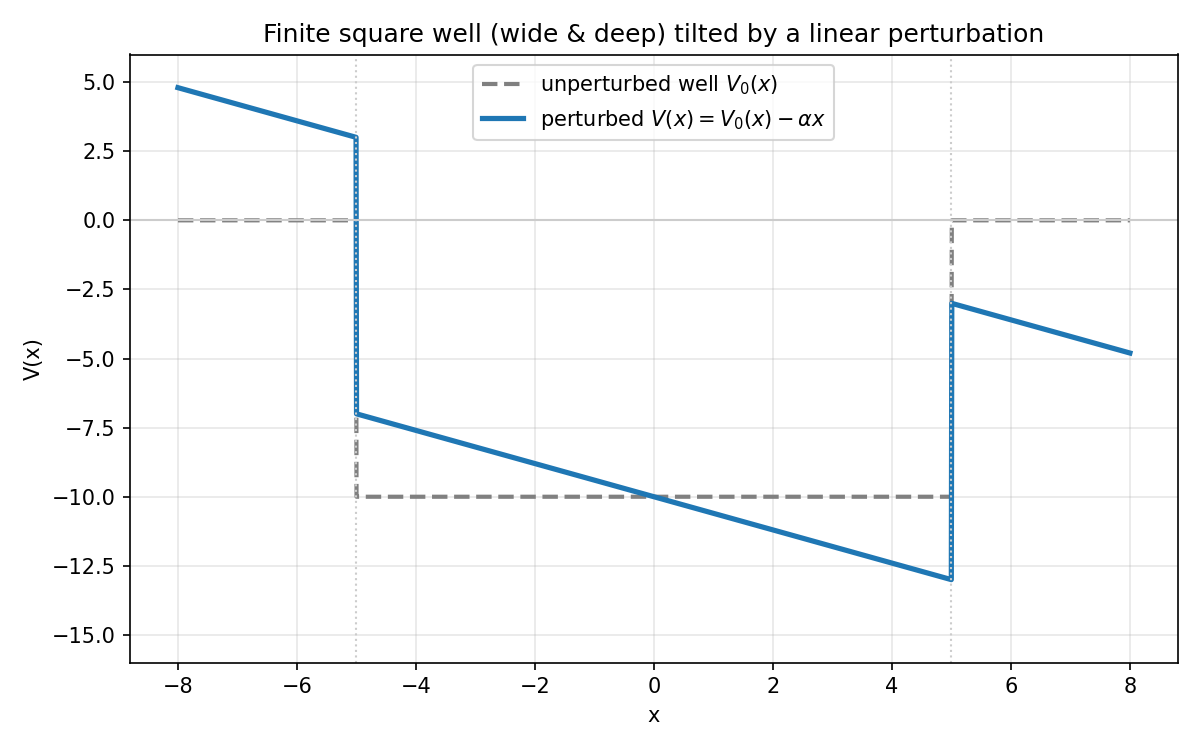
\includegraphics[width=0.8\textwidth,valign=t]{fig/sketch_tilted_well.png}
    \item 
    The barrier starts from $a$ to $\frac{1}{\alpha}\left[
    V_0-\frac{\pi^2\hbar^2}{8ma^2}
    \right].$
    \begin{align*}
        \gamma =& \frac{1}{\hbar}
        \int_a^{\frac{1}{\alpha}\left[
    V_0-\frac{\pi^2\hbar^2}{8ma^2}
    \right]}\sqrt{2m(-\alpha x +V_0-\frac{\pi^2\hbar^2}{8ma^2})}dx\\
    =&
    \frac{1}{\hbar}
    \frac{-2^{\frac{3}{2}} \sqrt{m} \left(-{\alpha}x - \frac{\pi^{2} h^{2}}{8a^{2} m} + V_{0}\right)^{\frac{3}{2}}}{3{\alpha}}
    \bigg|^{\frac{1}{\alpha}\left[
    V_0-\frac{\pi^2\hbar^2}{8ma^2}
    \right]}_a\\
    =&
     \frac{1}{\hbar}
    \frac{2^{\frac{3}{2}} \sqrt{m} \left(-{\alpha}a - \frac{\pi^{2} h^{2}}{8a^{2} m} + V_{0}\right)^{\frac{3}{2}}}{3{\alpha}}\\
    \approx &
     \frac{\sqrt{8mV_0^3}}{3\alpha\hbar}
    \end{align*}
    The kinetic energy is $\frac{\pi^2\hbar^2}{8ma^2},$ so the momentum is $\frac{\pi\hbar}{2a},$ thus 
    $$
    \tau = \frac{4a}{\frac{\pi\hbar}{2a}/m}e^{2\gamma}
    =\frac{8ma^2}{\pi\hbar}e^{2\gamma}.
    $$
    \item $$
    \gamma = 43640
    $$
    $$
    \tau\approx 10^{37882}yrs
    $$
    The age of the universe is $10^{10}yrs,$ so the tunneling in the Stark effect is not an issue.
    
    
\end{enumerate}

\subsection*{Sol. 19}
\begin{align*}
    \gamma = \frac{1}{\hbar}\int_0^{x_0}
    \sqrt{2m^2gx}dx
    =\frac{1}{\hbar}\sqrt{2m^2 g}\frac{2}{3}(\sqrt{R^2+(h/2)^2}-h/2)^{\frac{3}{2}}
\end{align*}
Estimate $R=3.3cm,$ $h=12.2cm,$ $m=380 g$ then $\gamma=8\times 10^{30}.$
$
v\approx 1.04\times10^{-10}m/s
$
$$
\tau \approx 20\times  e^{16\times 10^{30}} yrs.
$$

\subsection*{Sol. 20}
\begin{enumerate}
    \item 
    \begin{align*}
    Ae^{-ika}+Be^{ika}
    =\frac{1}{\sqrt{p(-a)}}
    [C_+e^{i\phi(-a)}+C_-e^{-i\phi(-a)}]
\end{align*}
\begin{align*}
   \frac{1}{\sqrt{p(a)}}
    [C_+e^{i\phi(a)}+C_-e^{-i\phi(a)}]
    =Ce^{ika}
\end{align*}
Since we assume that $V$ is analytic and vanishes when $|x|>a,$ $p'(\pm a)=0.$
\begin{align*}
    ikAe^{-ika}-ikBe^{ika}
    =&\frac{1}{p(-a)}
    [(i\phi'(-a)C_+e^{i\phi(-a)}-i\phi'(-a)C_-e^{-i\phi(-a)})\sqrt{p(-a)}]\\
    \Rightarrow
    kAe^{-ika}-kBe^{ika}=&\frac{1}{\hbar}(C_+e^{i\phi(a)}-C_-e^{-i\phi(a)})\sqrt{p(a)}
\end{align*}
\begin{align*}
    ikCe^{ika}
    =&\frac{1}{p(a)}
    [(i\phi'(a)C_+e^{i\phi(a)}-i\phi'(a)C_-e^{-i\phi(a)})\sqrt{p(a)}]\\
    \Rightarrow 
    kCe^{ika}=&\frac{1}{\hbar}(C_+e^{i\phi(a)}-C_-e^{-i\phi(a)})\sqrt{p(a)}
\end{align*}

Therefore
\begin{align*}
     Ae^{-ika}+Be^{ika}=Ce^{ika},\; Ae^{-ika}-Be^{ika} = Ce^{ika}
\end{align*}
\begin{align*}
    A = \frac{1}{2}Ce^{ika},\;
    B = 0.
\end{align*}
\item 
\begin{align*}
    p(iy)=&\sqrt{2m(E-V_0\operatorname{sech}^2(iy/a))}\\
    =&\sqrt{2m(E-\frac{4V_0}{e^{2iy/a}+e^{-2iy/a}+2})}\\
    =&\sqrt{2m(E-\frac{4V_0}{2\cos(2y/a)+2})}
\end{align*}
$$
\cos(2y_0/a)=\frac{2V_0}{E}-1
$$
$$
\tan^2(y_0/a)=\frac{1-\frac{2V_0}{E}+1}{1+\frac{2V_0}{E}-1}
=\frac{E-V_0}{V_0}
$$
\begin{align*}
    \lambda=&\frac{2}{\hbar}
    \int_0^{y_0}
    \sqrt{2mE-\frac{4mV_0}{\cos(2y/a)+1}}dy\\
    =&
    \frac{2}{\hbar}\sqrt{4mV_0}
    \left[
    \sqrt{\frac{E}{2V_0}} \, a \arctan\left(\frac{\sqrt{2} \sqrt{\frac{E}{2V_0}} \tan\left(\frac{y}{a}\right)}{\sqrt{-\tan^{2}\left(\frac{y}{a}\right) + 2\frac{E}{2V_0} - 1}}\right) - \frac{a \arcsin\left(\frac{\tan\left(\frac{y}{a}\right)}{\sqrt{2\frac{E}{2V_0} - 1}}\right)}{\sqrt{2}}
    \right]\bigg|^{y_0}_0\\
    =&
    \frac{2}{\hbar}\sqrt{4mV_0}
    \left[
    \sqrt{\frac{E}{2V_0}} \, a \frac{\pi}{2} - \frac{a}{\sqrt{2}}\frac{\pi}{2}
    \right]\\
    =&\frac{\pi a}{\hbar}(\sqrt{2mE}-\sqrt{2mV_0})
\end{align*}
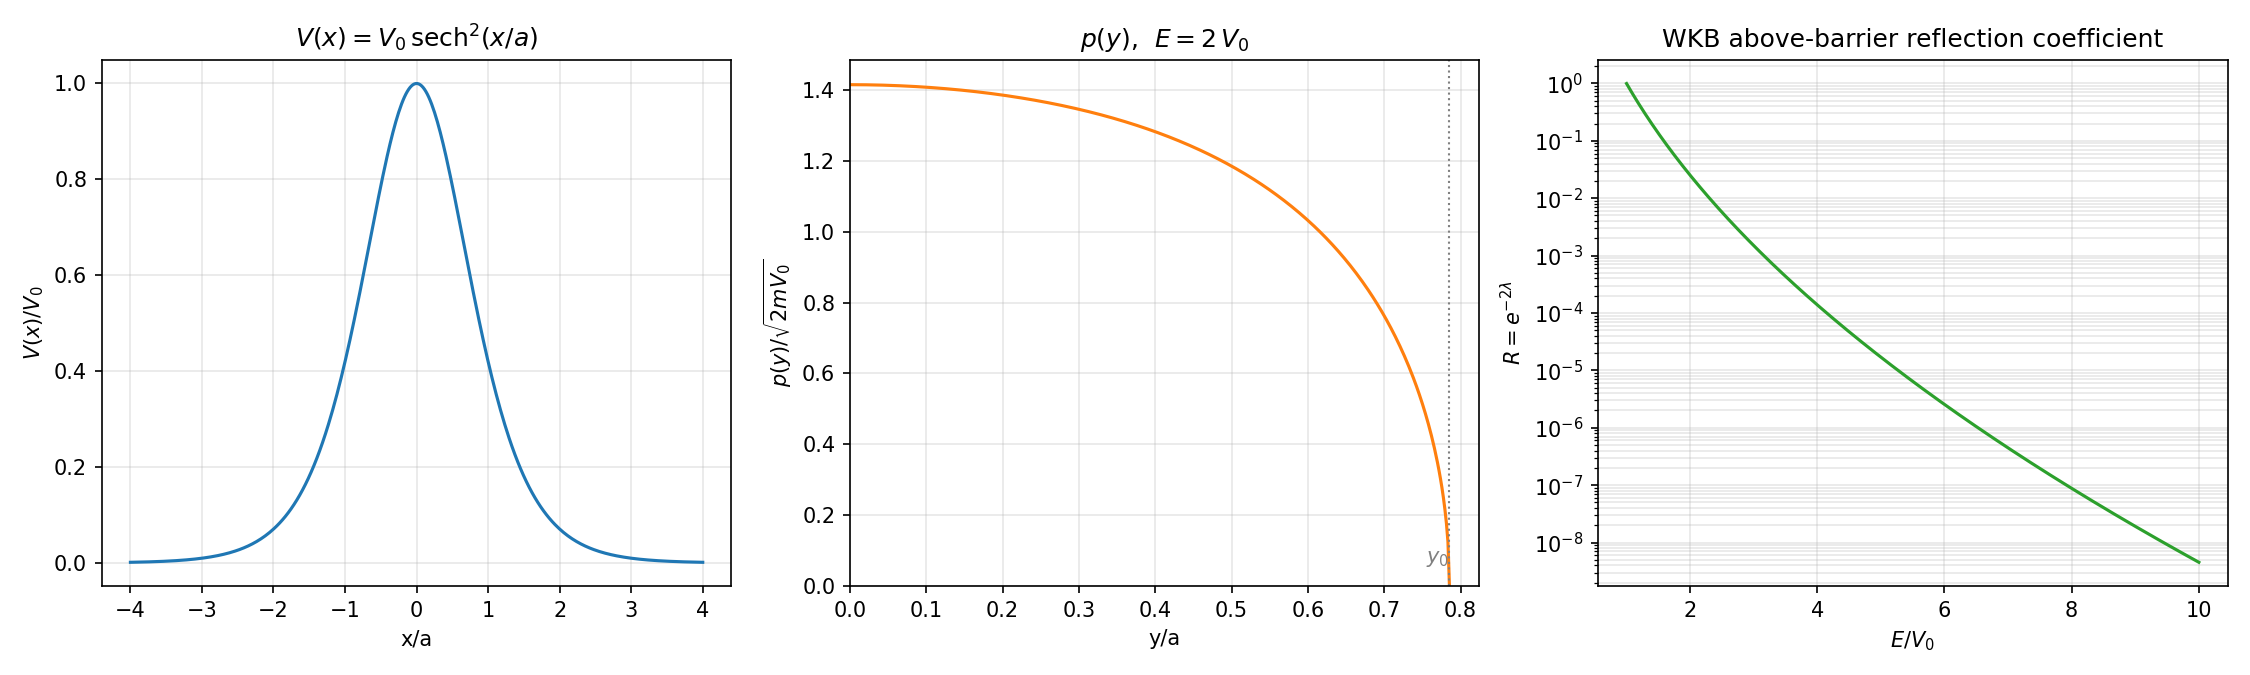
\includegraphics[width=0.8\textwidth,valign=t]{fig/prob9.20.png}
\item 
\begin{align*}
    \lambda =& \frac{2}{\hbar}
    \int_0^{y_0}
    \sqrt{2m(E - \frac{V_0}{1+(iy/a)^2})}dy\\
    =&
     \frac{2}{\hbar}
    \int_0^{y_0}
    \sqrt{2m(E - \frac{V_0}{1-(y/a)^2})}dy\\
    =&
    (2a\sqrt{2mE}/\hbar) [ E(k0) - (V_0/E)K(k_0) ],
\end{align*}
where $k_0 = \sqrt(1-V_0/E),$ and 
$K, E$ = complete elliptic integrals of the 1st/2nd kind, modulus k.

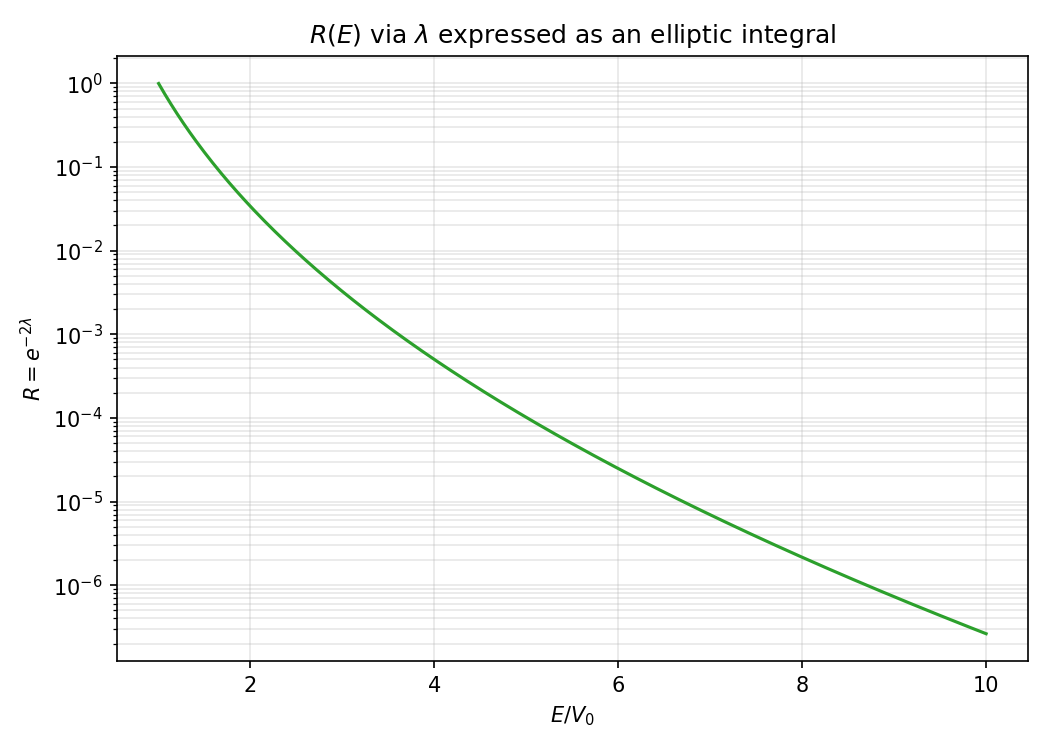
\includegraphics[width=0.8\textwidth,valign=t]{fig/prob9.20d.png}

\end{enumerate}

\subsection*{Sol. 21}
\begin{align*}
    \log_{10}\tau\ln2 
    = & \log_{10} \ln 2 +  \log_{10} \frac{2r_1}{v}e^{2\gamma}\\
    =&\log_{10} \ln 2 +  2(K_1\frac{Z}{\sqrt{E}}-K_2\sqrt{Z r_1})\log_{10}e+\log_{10} \frac{2r_1}{v}.
\end{align*}
The slope would be $-2K_1 Z\log_{10}e= -150.$ From $E = 5MeV$ to $6MeV,$ $\frac{-1}{\sqrt{E}}$ changes about $0.040MeV^{-1/2},$ thus the value of logarithm half life should decrease by $5.9,$ which matches the slope of the figure.